\chapter{Analysis and Design}
\label{chap:analysis-and-design}

%\bigskip

% \begin{table}[tb] % placement: h for here, t for top, b for bottom
%   \centering
%   \begin{tabular}{l c}  % two columns: l for left, c for center, r for right
%     Feature  & Benefit
%     \\\hline
%     Objects  & State encapsulation
%     \\
%     Generics & Code reuse
%   \end{tabular}
%   \caption{Advantages of Java}
%   \label{tab:java-advantages}
% \end{table}


The Analysis part of this chapter will outline what features the robot will have and discuss the 
pros and cons of the technologies researched. 
The Design part will cover the choices made during the analysis and the reasoning why.


\section{Machine Learning}
\label{sec:Machine Learning}

Machine learning is a subset of artificial intelligence
that focuses on the development of a computer program that learns from data.
In machine learning there are three approaches: supervised, unsupervised, and reinforcement learning.
Each of these approaches has its own strengths and weaknesses, but all of them need a machine learning algorithm.

A machine learning algorithm is a set of rules or mathematical
procedures that the system follows to learn from a dataset
and make predictions or decisions based on the data.

After applying the algorithm a dataset, you will have what is called a Machine learning Model.
A model is a specific instance of a trained system that has learned from the data and can make predictions or classifications.
\cite{ML-Models}
\textbf{Analogy:} A machine learning model is like a fully cooked meal.
The recipe (algorithm) was used to prepare it, but now it is a ready-to-use product.

\subsection{Supervised Learning}
The supervised learning approach is the more common approoach of the 3 approaches.
This is due to its ability to predict a wide range om problems accuratly,
however its effectiveness is dependent on the quality of the training data.
Supervised learning uses labled dataset to train the model,
which means that from the input data we expect the correct output data as well.
\cite{GoogleCloud-SL}

Some examples of supervised learning are spam email classifiers,
so wheter an email is spam or not and weather prediction models.

\subsection{Unsupervised Learning}
Unsupervised learning is a type of machine learning
that learns from data without human supervision. Unlike supervised learning,
unsupervised machine learning models are given unlabled data and allowed to discover patterns
and relationships without any explicit guidance or instructions. \cite{GoogleCloud-UL}

\subsection{Reinforcement Learning}
Reinforcement learning is the third type of machine learning.
Unlike the previous branches of machine learning,
reinforcement learning relies on a datasets with predefined answers, it learns by experience.
In reinforcement learning, an agent learns to achieve a goal in
an uncertain and potentially complex evironment/s py recieveing feedback
through rewards or penalties. \cite{RL-GeeksForGeeks}
\newline
The key concepts of reinforcement learning:
\begin{itemize}
      \item Agent: The learner/decision maker
            \begin{enumerate}
                  \item An agent is anything that can be viewed as percieving its environment through
                        sensors and acting upon that environment and as mentioned above, the agent is the learner/decision maker because it
                        learns from its environment and makes decisions based on what it has learned.
                        For a software agent the sensors could be the input data, network packes or keystrokes
                        and the actuators are the output data. \cite{IntelligentAgents}
            \end{enumerate}
      \item Environment: Everything the agent interacts with. The environment is the context in which the agent acts opun and learns from,
            and there exists a lot of different environment types. \cite{IntelligentAgents}
            \begin{enumerate}
                  \item Deterministic vs Stochastic is the part of the environment that determines if the next state is completly
                        determined by the current state and agents action or if there is some randomness involved.
                  \item Episodic vs Sequential describes wheter the agents experience is divided into unconnected episodes or
                        if the agents actions have long-term consequences on the environment.
                  \item Static vs Dynamic is wether the environment can change while the agent is making a decision.
                  \item Discrete vs Continuous is the number of possible actions and states the environment can provide the agent.
                  \item Single-Agent vs Multi-Agent is the number of agents operating in the same environment.
            \end{enumerate}
      \item State: A specific situation the agent finds itself in.
      \item Actions: What possible moves the agent can make.
      \item Rewards: Feedback from the environment, that helps guide the learning process.
      \item Policy: The agent's strategy for decision making.
      \item Value Function: Predicts future rewards of a state and/or action.
      \item Exploration vs Exploitation: Balancing between trying new action or using known best actions.
\end{itemize}


\subsubsection{Types of Reinforcement Learning Agents}
And even in reinfocement learning there exists subsets of algorithms that can be used, where
the two main types of reinforcement learning algorithms:
\begin{itemize}
      \item Model-Free Reinforcement Learning: Uses experience to learn directly from one or both of simpler quantities, state/action value-functions or policies.
      \item Model-Based Reinforcement Learning: Uses experience to construct an internal model of the 
      transitions and immediate outcomes in the environment.
\end{itemize}

\paragraph{Model-free Reinforcement Learning}
Model-free methods bypass the need for an environmental model and instead
learns a policy or value function directly through interactions. These metehods
can generally be simpler to implement but often, require a lot more training data 
and memory to store Q-tables for large environments.
Value-based methods, focus on the learning of a value function that estimates 
the expected return (cumulative reward) from a given state or state-action pair.
\begin{itemize}
      \item Q-learning is on of these value-based methods, and is an off policy algorithm,
      that learns the optimal action-value function \(Q*(s,a) \). The agent updates the 
      Q-values using to Bellman's equation: \cite{Types-of-Reinforcement-Learning}
      \begin{equation}
            Q(s,a) \leftarrow Q(s,a) + \alpha [r + \gamma \max_{a'} Q(s',a') - Q(s,a)]
      \end{equation}
      \item SARSA or State-Action-Reward-State-Action is an on-policy method that 
      updates Q-values based on the current policy. \cite{SARSA}
      \begin{equation}
            Q(s,a) \leftarrow Q(s,a) + \alpha [r + \gamma Q(s',a') - Q(s,a)]
      \end{equation}
      \item Deep Q-Networks (DQN) combines Q-learning with deep neural networks 
      to handle more complex environments with large state spaces. This approach leverages deep learning 
      to approximate Q-values. \cite{Types-of-Reinforcement-Learning}
\end{itemize}

Policy-based methods, on the other hand learn a policy direcly without estimating
value functions. They are usefull in continuous action spaces and stochastic policies.
\begin{itemize}
      \item REINFORCE is on one such policy and is a Monte Carlo policy gradient methods, 
      that optimizes the policy by adjusting probability of taking actions that lead to a 
      higher cumulative reward. The policy is updated accoding to the gradient of expected rewards,
      where \(\mathbb{R}\) is the cumulative reward. \cite{Types-of-Reinforcement-Learning}
      \begin{equation}
            \nabla J(\theta) = \mathbb{E} \left[\nabla \log \pi_{\theta}(s_t,a_t) R_t \right]
            \label{equation:policy_gradient}
      \end{equation}
      \item Actor-critic methods, combine both the policy learning (actor) with a value
      function estimator (critic) for a more stable learning process. \cite{Types-of-Reinforcement-Learning}
      \item Proximal Policy Optimization (PPO) is an improvement upon the basic policy
      gradient methods. It uses a clipped objective function to limit the amount of policy 
      changes, to prevent drastic cnages during training, and thus improving stability. \cite{Types-of-Reinforcement-Learning}
\end{itemize}
Some disadvantages of policy-based methods is they have a high variance in gradient estimates and often requires careful 
tuning of learning rates and other hyperparameters. \cite{Types-of-Reinforcement-Learning}

\paragraph{Model-Based Reinforcement Learning}
Model-based RL aims to learn a model of the environment's transitions dynamics
and reward function. Once a model is accurate enough, it can be used to 
simulate trajectories and plan ahead, making an agent learning significantly more
sample efficient. There are two main approaches to model-based RL \cite{ReinforcementLearning}:
\begin{itemize}
      \item Learn the model 
      \item Given a model
\end{itemize}
Typically, model-based agents has a model of the environment, a planner function that uses
the model to search for optimal actions (e.g., via tree search or Optimization), and a policy
that may be learned directly or indirectly through planning.
Some types of model-based methods are:
\begin{itemize}
      \item Dyna Architecture (Sutton) that combines learning from lear experiences, 
      with a simulated planning from the learned model.
      \item Monte Carlo Tree Seach (MCTS) which is used in conjunction with learned models
      to plan moves by simulating possible future states (Notably used in AlphaGo). \cite{ReinforcementLearning}
      \item Model predictive Control (MPC), is a planning based method, where the agent
      uses a learned or predefined model to predict a few stepts in the environment and 
      selcts the action that optiomizes the cumulative reward function over a planning horizon. \cite{Types-of-Reinforcement-Learning} 
\end{itemize}
The drawbacks of model-based methods is that altough they can have more assumptions
and approximations on a given task, but they may only be limited to that sepcific 
type of task. It also requires accurate models of the environment and building a model
can be computationally difficult and expensive and therefore lead to inaccuracies. \cite{Types-of-Reinforcement-Learning}

\subsection{Design Decision: Machine Learning Approach}
\label{sec:ML-Design-Decision}
In the designing of the machine learning model for this project, three core learning paradigms
were considered: Supervised learning, unsupervised learning and reinforcement learning. Each 
approach offers distinct advantages and challenges, but given the problem domain and 
project goals, reinfocement learning was ultimatly selected as the most appropriate method.

\textbf{Supervised learning}, is a powerfull approach that is known for its high accurarcy when trained on
suffeciently large and labeled datasets. However, its not well-suited to this project for
two main reasons. Firstly, aquiring a large and detailed labeled dataset for pokemon battles
would be impractical and time-consuming. Secondly, supervised models are static in nature, they learn
from pre-exisiting data and do not adapt during deployment. Since this project aims to develop
an autonomous agnet, interact with and improve through the ever evolving environment of pokemon battles, 
these limitations made supervised learning an unsuitable choice.

\textbf{Unsupervised learning}, while advantageous in situations where data is unlabeled, is primarily
geared towards pattern discovery and clustering. As such, it lacks the ability to learn 
optimal behavior through interaction and feedback. Given the goal of this projects agent is not
merely to identify patterns, but actively engage in all kinds of battles and make sequential decisions,
unserpervised learning was deemed unsuitable.

\textbf{Reinforcement learning}, by contrast offers a framework where an agent learns through direct interaction
with an enviromnent by performing actions and recieveing feedback in the form of rewards or penalties.
This alligns closely with the nature of the normal pokemon battle system, which is sequential, 
turn-based and goverend by strategic decision making. Reinforcement learning allows the agent to
adapt and imrpove over time through trial and error, making it a well-suited choice for this project.

Having established that reinforcement learning as the preferred approach, a specific algorithm
was selected to implement the agent's learning mechanism. The algorithm chosen is the 
Deep Q-Network (DQN). DQN was selected for a couple of reasons. Firstly it supports discrete 
action spaces, which aligns well with pokemon battles, where action (moves, switches ect.) are
clearly defined and finite. Second, DQN is capable of learning from raw numerical representations
of state data, allowing for efficient learning from the complex state space of pokemon battles.
Finallu, the use of experience replay and a target network, which are two core components of DQN, 
helps improve training stability and sample efficiency, which is crucial given computational constraints
and training duration of this project.
\section{Choice of language}
\label{sec:choice-of-language}

\subsection{Python}
\subsection{C++}
\subsection{JavaScript}
\subsection{Unity with C\#}

\section{Data source}
\label{sec:data-source}

In order to simulate a Pokemon battle, it is necessary to have the data needed for a Pokemon battle to take place.
The simulator needs data on Pokemon species and their stats and moves, as well as data on what the individual moves do.
It needs to know about Pokemon abilities and held items, and how they interact with eachother.

To this end it is important to find a good data source to work with. The following are some options to consider
for this purpose.

\subsection{Data mining}
Data mining is the process of discovering patterns in large data sets \cite{DataMining}. It is commonly used in video games to extract raw data 
from game files, such as assets (3D models, sprites, etc.) or hidden details of how certain functions interact in a game. This data has historically
been used for online documentation of game mechanics \cite{DataMiningPokemon} or even for creating fan-made modifications to the original game \cite{RenegadePlatinum}.

For the purpose of creating a battle simulator, it would be possible to "mine" the data directly from the game files. This is a lengthy process, however
and can be viewed as a grey area in terms of legality or ethicality. This is because it involves sideloading software on a physical console in order to
extract encrypted data from both the console and the game cartridge itself. Once in possesion of the keys and game data, it is then possible to extract
data by removing multiple layers of encryption and parsing Nintendo's proprietary file formats.

This method would be the most accurate data source available, but is also the most tedious option to use compared to other data sources.

\subsection{Kaggle}
\subsection{PokeAPI}



% \begin{figure}[tb] % placement: h for here, t for top, b for bottom
%   \centering
%   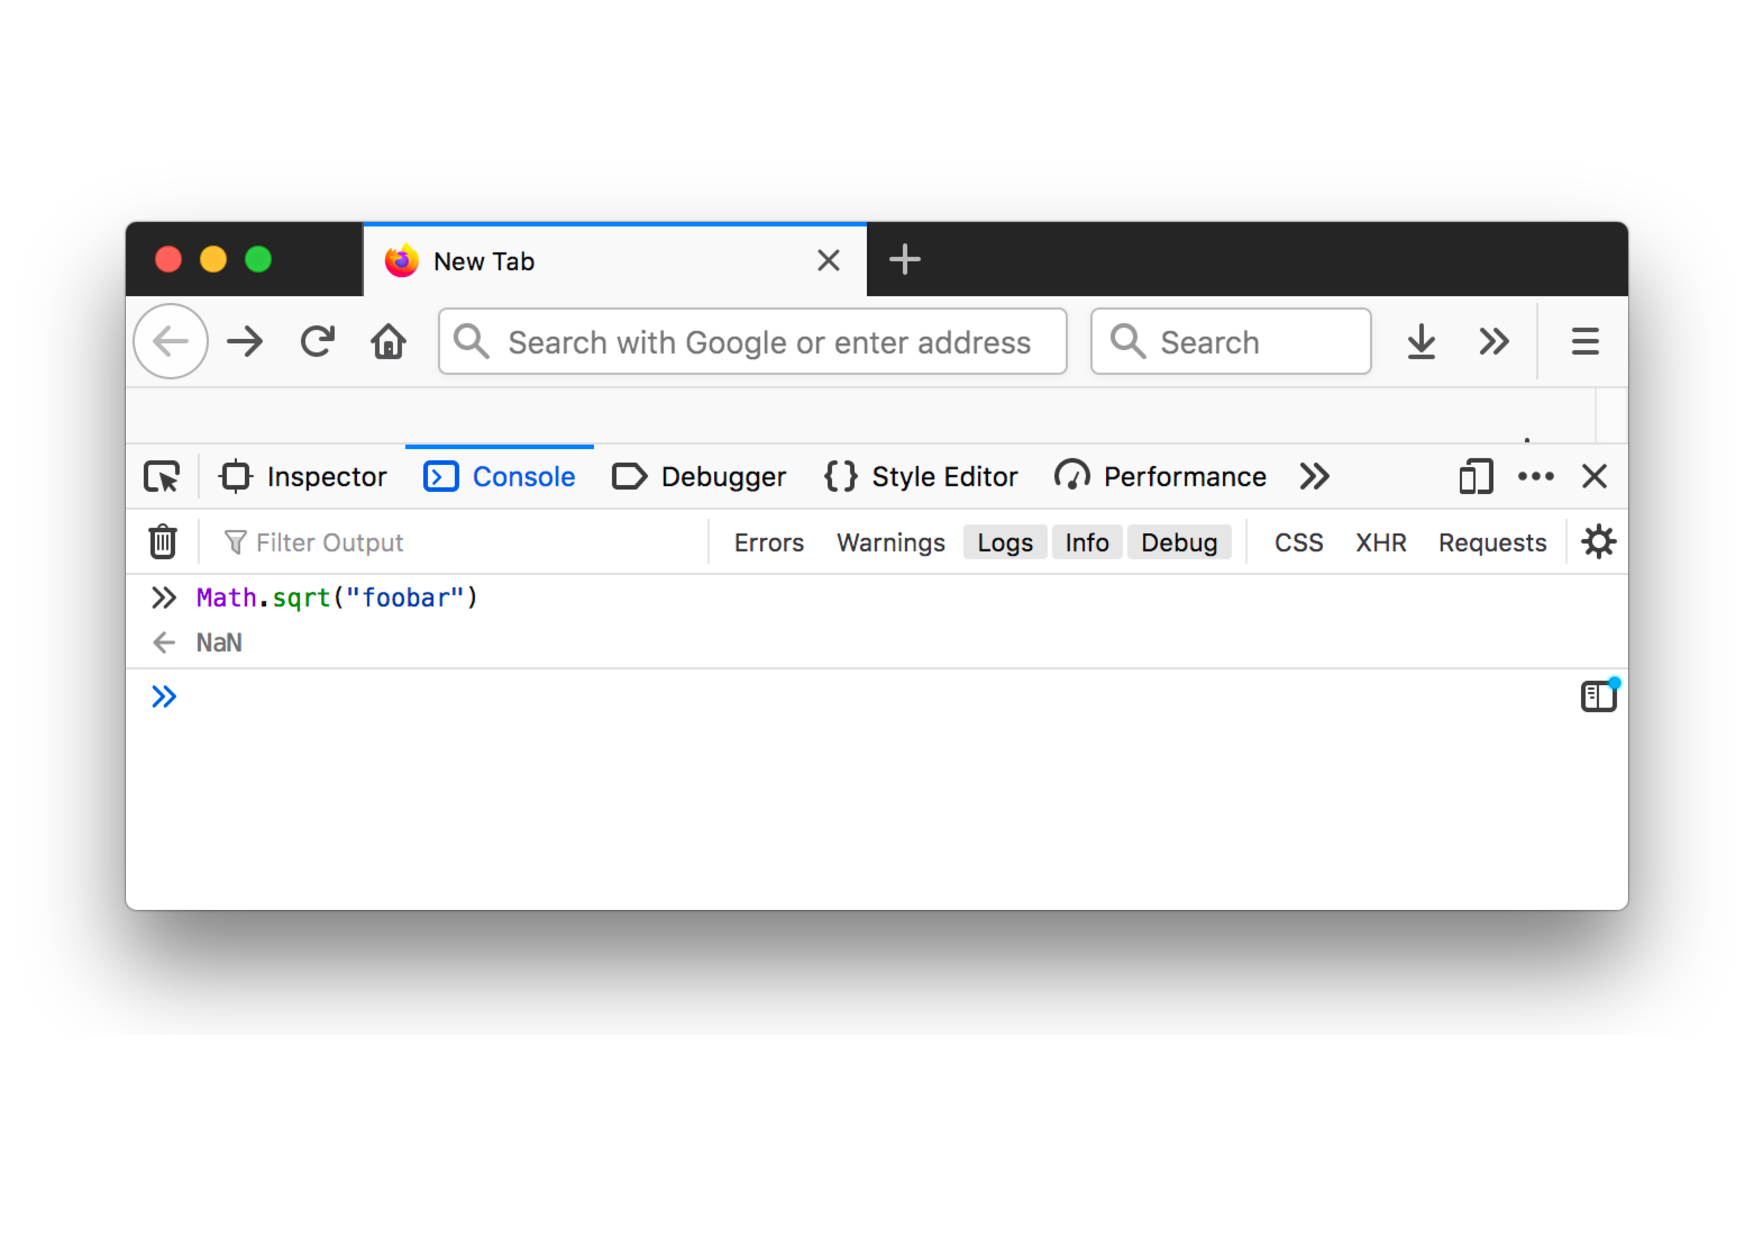
\includegraphics[width=.9\linewidth]{assets/firefox-js-console}
%   \caption{The JavaScript console in Firefox }
%   \label{fig:firefox-js-console}
% \end{figure}
